\documentclass[12pt]{article}
\usepackage[utf8]{inputenc}
\usepackage{graphicx}
\usepackage[letterpaper, top = 2 in, right = 1.2in, left = 1.2 in, bottom = 1 in,  headheight=95pt, headsep=30pt]{geometry}
\usepackage{setspace}
\usepackage{titlesec}
\usepackage{fancyhdr}
\usepackage{caption}
\usepackage{tikz}
\usepackage{graphicx}
\usepackage{setspace}
\usepackage{tabularx}
\usepackage{eso-pic}
\usepackage{xcolor}
\usepackage{amsmath}
\usepackage{amssymb}
\usepackage[backend = biber, style = apa]{biblatex}
\addbibresource{references.bib}

% Customization
% Document Customization
\setlength{\parindent}{0.5 in}
\titleformat{\section}[block]{\doublespacing\bfseries\centering}{}{0pt}{}
\titleformat{\subsection}[block]{\doublespacing\bfseries}{}{0pt}{}
\titleformat{\subsubsection}[block]{\doublespacing\bfseries}{}{0pt}{}
\titleformat{\subsubsubsection}[block]{\doublespacing\bfseries}{}{0pt}{}

\newcommand{\verticallineinmargin}{
    \AddToShipoutPictureBG*{
        \AtPageLowerLeft{
            % Adjust the positions and lengths of the lines here
            \put(72,0){\line(0,1){842}}  % Left margin line
            \put(540,0){\line(0,1){842}} % Right margin line
        }
    }
}

\newcommand{\horizontallinemargin}{
    \AddToShipoutPictureBG*{
        \AtPageLowerLeft{
            \put(0, 60){\line(1, 0){700}}
            \put(0, 710){\line(1,0){700}}
            \put(0, 685){\line(1,0){700}}
            \put(0, 35){\line(1,0){700}}
        }
    }
}

% Header and Footer Customization
\pagestyle{fancy}
\fancyhf{}
\fancyhead[C]{
    \verticallineinmargin
    \horizontallinemargin
    \protect\begin{minipage}{\textwidth}
        \centering
        \includegraphics[width = 50pt]{PUPLogo.png} \\
        \vspace*{0.6 cm}
        \textbf{POLYTECHNIC UNIVERSITY OF THE PHILIPPINES}
    \end{minipage}
}
\fancyfoot[C]{\thepage}
\renewcommand{\headrulewidth}{0pt}

\begin{document}
\begin{titlepage}
    \thispagestyle{fancy}
    \fancyfoot[C]{\textcolor{white}{\thepage}}
    \centering
    \vspace*{2cm}  % Adjust vertical space from the top
    \textbf{Linear and Quadratic Discriminant Analysis of Alzheimer's and Non-Alzheimer's Patients
    Based on Lifestyle Factors, Clinical Measurements, and Cognitive and Functional Assessments}
    
    \vspace*{4cm} 
    \normalsize
    In partial fulfillment of the requirements in \\ 
    STAT 20253: Multivariate Analysis

    \vspace*{3cm}
    By \\ [0.5 cm]
    Almer John Sta. Ines \\ [0.3 cm]
    Dencie Mae Saguano \\ [0.3 cm]
    Jerolle Nonato \\ [0.3 cm]
    Joy Ellen Mae Yangyang \\ [0.3 cm]
    Juan Raphael Pimentel \\ [0.3 cm]
    Roldan Libay Jr. 
    \vfill
    \textbf{2025}
\end{titlepage}

% Table of Contents
\newgeometry{top=2in, bottom=1in, left=1.2in, right=1.2in}
\renewcommand{\contentsname}{TABLE OF CONTENTS}
\pagenumbering{roman}
\doublespacing
\tableofcontents

% Chapter 1
\restoregeometry

\pagenumbering{arabic}
\setcounter{page}{1}

\newpage

\section{CHAPTER I \\ THE PROBLEM AND ITS SETTING}
\doublespacing
\noindent

This chapter contains the introduction, statements of the problem, research hypothesis, 
significance of the study, scope and limitations, and definition of terms. 

% Introduction
\subsection{Introduction}
\noindent

Every three seconds, someone in the world develops dementia, adding to the more than 55 million people already 
living with the condtion as of 2020 (\cite{alzint_dementia_statistics}). This number is expected to nearly double 
every 20 years, reaching 78 million in 2030 and a staggering 139 million by 2050. Alzheimer's disease (AD) the most
common cause of dementia, is a progressive brain disorder that gradually affects memory, thinking skills, and the ability
to carry out everyday tasks (\cite{AlzheimersAssociation2021}). As the prevalence of AD continues to rise, it affects people not only altering their lives 
but also placing an emotional and financial strain on families and healthcare system. Early detection is crucial as it allows for 
timely interventions, potential treatments, and better supportfor both patients and caregivers (\cite{Dubois2016}). However, diagnosing AD in its early stages remains challenging, 
as its symptoms often overlap with other cognitive conditions, making it difficult to distinguish from normal aging or mild cognitive impairment (\cite{Jack2018}). Understanding the key
indicators of AD can help improve early diagnosis and lead to better patient outcomes.

A study by Livingston et al. (2020) suggests that lifestyle factors, medical history, clinical measurements, and cognitive and functional assessments can provide essential insights into the
early idenitifaction of Alzheimer's disease. Lifestyle factors, such as Body Mass Index (BMI), smoking status, alcohol consumption, physical activity, diet quality, and sleep quality can impact 
the risk of developing AD (\cite{nih_healthy_lifestyle}). Additionally, certian medical conditions, including hypertension, diabetes, cardiovascular, diseases, depression, family history of AD, and
head injury have been linked to increased susceptability to AD (\cite{Kivipelto2018}). Clinical measurements, particularly cardiovascular health indicators, have been increasingly recognized as significant
risk factors for the disease. Moreover, a study conducted by Leszek et al. (2020) suggests that cardiovascular diseases can contribute to the development and progression of AD by impairing blood flow to the brain
and causing inflammation (\cite{Leszek2021}). Functional assessments, which evaluate how well a person can manage daily tasks and adjust to cognitive changes, can also be an important tool in detecting early signs of AD. (\cite{sperling2011})

The effectiveness of classification models in predicting AD is crucial for developing reliable diagnostic tools. LDA and QDA are two widely used statistical techniques for classification problems. LDA assumes equal covariance structures
among groups, making it more effective when the assumption holds, while QDA relaxes this assumption, allowing for more flexibility in classification (\cite{elements_statistical_learning})

The study aims to investigate significant differences between Alzheimer's patients and Non-Alzheimer's patients concerning lifestyle factor, clinical measurements, and cognitive and functional assessments. Additionally, it seeks to identify 
substantial indicators of AD and compare the discriminative power of LDA and QDA in early prediction. By analyzing there aspects, this research contributes to the development of more accurate and efficient classification models for early AD 
diagnosis. 

\subsection{Objectives}
\noindent

The general objective of the study is to accurately discriminate Alzheimer's patients to Non-Alzheimer's patients based on their lifestyle factors, clinical measurements, and cognitive and functional assessment.

Specifically, it aims to achieve the following objectives. 

\begin{enumerate}
    \item To identify which clinical indicators can effectively discriminate Alzheimer's patients to Non-Alzheimer's patients. 
    \item To optimize a discriminant classification model through feature reduction. 
    \item To compare the discriminative power of LDA and QDA for an early prediction of AD. 
\end{enumerate}

\subsection{Statements of the Problem}
\noindent

Following the mentioned objectives, the study sought to answer the following questions. 
\begin{enumerate}
    \item Are there significant differences between Alzheimer's and Non-Alzheimer's patients in terms of:
    \begin{enumerate}
        \item Lifestyle Factors
        \item Clinical Measurements
        \item Cognitive and Functional Assessment
    \end{enumerate}
    \item What are the substantial indicators of AD? in terms of: 
    \begin{enumerate}
        \item Lifestyle Factors
        \item Clinical Measurements
        \item Cognitive and Functional Assessment
    \end{enumerate}
    \item How do the discriminative powers of LDA and QDA compare in the early prediction of AD?
\end{enumerate}

\subsection{Significance of the Study}
\noindent

This research aims to develop a classification model for the early prediction of AD by analyzing key factors such as lifestyle, clinical measures, and cognitive and functional assessments. 
The findings of this study will be significant to the following sectors: 

\textbf{Healthcare Practitioner and Neurologist}. This study will provide a data-drive aproach for early AD prediction, aiding in timely intervention and personalized treatment plan. Furthermore, 
this research will enhance the understanding of the most substantial indicators of AD based on statistical multivariate models. 

\textbf{Researchers and Data Scientist}. The study will contribute to the growing field of medical data analysis by exploring the effectiveness of LDA and QDA in disease membership classification. It 
will serve as a foundation for the future studies integrating machine learning and statistical methods in healthcare analytics which will potentially lead to more advanced diagnostic tools. 

\textbf{Patients and Families}. This study will benefit them as early detection tools can help them prepare for disease management and necessary lifestyle adjustments. This will also raise awareness of the 
key lifestyle and medical factors that may contribute to the risk of AD and encourage them to have preventive measures that may delay the onset of disease.

\textbf{Public Health and Policy Makers}. This study holds significance to the general public health sector by supporting the development of data-drive healthcare policies focused on early screening and intervention
programs. The insights gained from this research can help allocate resources in AD research, prevention and treatment programs.

\subsection{Scopes and Limitations}
\noindent

This study aims on developing a classification model for early prediction of AD using LDA and QDA. It focuses on analyzing and identifying important factors such as lifestyle habits, clinical measurements, and cognitive and 
functional assessments to distinguish between Alzheimer's and Non-Alzheimer's patients. The study also compares the discriminative power of LDA and QDA in identifying substantial predictors of the disease and compares their 
classification performance. 

The dataset used in this study consists of 2,149 patient records with unique identifications ranging from 4571 to 6900. It includes demographic details, lifestyle factors, medical history, clinical measurements, cognitive and functional
assessments, symptoms, and Alzheimer's diagnosis. Since the dataset is synthetically generated and designed from educational purposes, it provides a structured and controlled environment for analysis. However, because it is not based on real patient data, 
it may not fully capture the variability and complexity of real-world medical dataset. 

Despite its strengths, the study has certain limitations. Since the dataset is synthetic and not sourced from actual medical records, the generalizability of the findings to real-worlc clinical settings may be restricted. Additionally, LDA and QDA rely on certain
statistical assumptions, like normality and homoscedasticity for LDA, which may effect their predictive accuracy in more complex datasets. This study also does not compare LDA and QDA with other machine learning models, limiting the analysis to just these two multivariate
techniques. 

\subsection{Defintion of Terms}

\newpage
\section{CHAPTER II \\ REVIEW OF LITERATURE AND STUDIES}

\subsection{Factors Influencing Alzheimer's Disease}
\subsubsection {Lifestyle Factors}
\noindent

Lifestyle behaviors play a vital role in maintaining cognitive health and reducing the rish of Alzheimer's disease. Engaging in regular physical activity, for instance, has been linked to a lower likelihood of cognitive decline. \cite{Dominguez2021} emphasized that aerobic
exercises not only boost brain function but can also help delay the onset of dementia. Similarly, following a healthy diet, particularly one rich in fruits, vegetables, and whole grains, like the Mediterranean diet, has been shown to enhance cognitive performance and decrease
the risk of Alzheimer's. Maintaining an active social life also contributes significantly, as frequent social interactions and participation in activities foster cognitive resilience and lower the chanves of developing dementia. (\cite{Dominguez2021})

Sleep quality and duration are emerging as important factors in Alzheimer's risk. Poor sleep habits, such as not getting enough rest or experiencing disrupted sleep, have been linked to a buildup of amylod-beta in the brain, a hallmark of Alzheimer's. \cite{Dominguez2021} highlights
that good-quality sleep is essential for brain health. It helps clear out metabolic waste products and supports memory consolidation, making it a critical part of maintaining cognitive function.

\subsubsection{Clinical Measurements}
\noindent

Recent advancements in biomarker research have greatly improved the ability to classigy and detect Alzheimer's disease at an early stage. Blood-based biomarkers, such as specific microRNAs (miRNAs), are showing promimse in identifying individuals at risk even before symptoms appear 
(\cite{JAMA2019}). Genetics also play a key role,, with the APOE4 allele being a well-known risk factor. People who carry this variant have a higher chance of developing Alzheimer's, and integrating genetic information into classification models can enhance accuracy in predicting the
disease (\cite{JAMA2019}).

Health conditions like diabeetes, heart disease, and high blood pressure have been linked to a higher risk of developing Alzheimer's disease. These issues can worsen the impact of vascular problems on brain function and may even interact with Alzheimer-related changes in the brain. Taking
steps to manage these conditions through healthy lifestyle choices and medical treatments, play a key role in lowering the overall risk of dementia (\cite{PMC2021}).

\subsubsection{Cognitive and Functional Assessment}
\noindent

Cognitive tests play a crucial role in identifying and classifying Alzheimer's disease. Standatd assessments like the Mini-Menteal State Examination (MMSE) and the Montreal Cognitive Assessment (MoCA) help measure cognitive function in a structured way. The results from these tests provide 
valuable insights that can improve classification models, making it easier to distinguish between healthy individuals, those with mild cognitive impairment, and those with Alzheimer's disease (\cite{PMC2021}). Functional assessment, on the other hand, focuses on understanding how well a person
can handle everyday tasks and adapt to changes in their thinking abilities. Tools like the Alzheimer's Disease Cooperative Study-Activities of Daily Living Inventory (ADCS-ADL) and the Functional Activities Questionnaire (FAQ) are often used to evaluate these abilities (\cite{Custodio2022}). Supported by
the study of \cite{Cummings2017} which stated that these assessments go beyond cognitive tests, offering a more complete picture of how Alzheimer;s disease affects a person's overall functioning and quality of life.

\subsection{Detection of Alzheimer's Disease using Discriminant Models}
\noindent

Linear Discriminant Analysis (LDA) and Quadratic Discriminant Analysis (QDA) are commonly used classification techniques in medical datasets, particularly for AD. According to \cite{jain2022}, LDA stands out for its simplicity, especially when data is linearly seperable, while QDA
handles more complex, non-linear patterns effectively but at a higher computational cost. This makes the choice between the two methods dependent on the nature of the dataset.

Recent research emphasizes the strengths of both approaches. LDA is praised for its ease of interpretation and ability to identify key predictors, offering reliable and computationally efficient models. In contrast, QDA, with its ability to handle non-linearities, excels in sensitivity, especially in
detecting early cognitive decline, but may sacrifice some interpretability (\cite{arbabshirani2017}). Studies show that LDA often has higher specificity, whereas QDA is more sensitive in distinguishing between healthy individuals and those with Alzheimer's (\cite{nguyen2020}).

Model interpretability and computational complexity remain critical considerations. LDAs straightforward structure allows for a better understanding of variable relatkionships, making it a practical choice in clinical settings. On the other hand, QDA's flexibility can come at the cost of higher
computational demands and reduced clarity in variable significance (\cite{wang2018}).

\subsubsection{Linear Discriminant Analysis (LDA)}
\noindent
LDA was used as a classification method to predict Alzheimer's disease patients based on clinical biomarkers, neuroimaging data, and metabolic profiles. This technique has been utilized in several studies to enhance diagnostic accuracy and distinguish between Alzheimer's disease, mild cognitive impairment
(MCI), and healthy controls. Data records mainly consisted of medical imaging data, metabolic biomarkers, and cognitive assessment scores, which were processed through feature selection and dimensionality reduction teechniques to enhance classification performance.

LDA assumes that different classes (AD and non-AD groups) share the same covariance structure and constructss linear boundaries to maximize class separability. In the study by (\cite{le2020_lda_highdimensional}), an adapted LDA approach was implemented to handle high-dimensional medical datasetss, ensuring better feature selection and
classification accuracy. Similarly, \cite{salasgonzalez2010_factor_analysis_lda} utilizied LDA in combination with factor analysis to select the most relevant features from 18F-FDG PET images, optimizing classification between Alzheimer's and control groups.

The study by \cite{yilmaz2021_metabolic_biomarkers_ad} applied artificial intelligence and machine learning techniques alongside discriminant analysis to identify biomarkers associated with Alzheimer's progression. Feature selection was crucial in reducing redundancy and enhancing predictive capability. \cite{maroco2011_data_mining_dementia}
conducted a comparative analysis between LDA, logistic regression, neural networks, support vector machines, classification trees, and random forests. They assessed model performance using key evaluation metrics, demonstrating that LDA achieved high accuracy in distringuishing AD patients from controls when optimized with feature selection.

\subsubsection{Quadratic Discriminant Analysis (QDA)}
\noindent

QDA, unlike LDA, relaxes the assumption of shared covariance struvtures and allows each class to have its own covariance matric, making it suitable for datasets where feature dsitributions exhibit non-linearity. This flexibility enables QDA to better handle complex biomarker distributions in Alzheimer's disease classification.

QDA has demonstrated strong classification performance in Alzheimer's research. Studies such as \cite{zhang2017_qda_neuroimaging} and \cite{pereira2020_qda_mri} explored the application of QDA in neuroimaging-based Alzheimer's diagnosis, showing that its ability to model class-specific covariance matrices led to improved classification precision
and recall. Additionally, the work of \cite{maroco2011_data_mining_dementia} indicated that QDA often achieved higher F1-scores in datasets with more complex patterns compared to LDA.

Furthermore, studies have shown that QDA performs well in scenarios where biomarker distributions exhibit high variability. For instance, \cite{lee2015_qda_mri_biomarker} demonstrated that QDA outperformed LDA in identifying Alzheimer's subtypes based on MRI-deived biomarkers, particularly in cases with overlapping clinical features. Similarly, 
\cite{garciarodriguez2016_qda_csf} employed QDA to analyze cerebrospinal fluid biomarkers, showing significant improvements in classifying AD and MCI patients. The higher Area Under the Curve (AUC) values reported in these studies suggest that QDA provides superior discrimination between AD and non-AD cases when biomarker variability is high.

\subsection{Feature Selection Techniques in Discriminant Analysis}
\subsubsection{Recursive Feature Elimination (RFE)}
\noindent

RFE is a backward feature elimination technique that iteratively removes the least significant features based on their impact on model accuracy. This study implements RFE to systematically refinea feature subsets, ensuring that only the most releveant biomarkers contribute to classification. The process starts by training an initial model on all features,
ranking their importance, and recursively eliminating the least informative ones until an optimal subset remains.

Previous studies, such as \cite{balakrishnan2020_rfe_ann_ad}, combined RFE with artificial neural netwroks to identify critical features for Alzheimer's disease classification. Similarly, \cite{alshamlan2018_biomarker_gene_selection} demonstrated that RFE facilitates biomarker gene selection, improving classification peformance. In this study, RE is applied
to clninical biomarkers, cognitive scores, and neuroimaging markers to eliminate redundant features, refine the input space, and mitigate overfitting, thereby enhancing the performance of LDA and QDA.

\subsubsection{Lasso Regression}
\noindent

Lasso regression, a form of regularization, employs an L1 penalty constraint to shrink the coefficients of less relevant features to zero, effectively selecting only the most significant predictors. This study applies Lasso regression to ensure that the discriminant functions of LDA and QDA are derived from the most influential biomarkers while minimizing
noise and improving model generalizability.

\cite{gu2020_feature_selection_ad} evaluated Lasso regression as a feature selection method for Alzheimer's diagnosis, emphasizing its capacity to identify high-impact features while preserving interpretability. Additionally, \cite{spooner2020_ensemble_feature_selection} demonstrated Lasso's efficacy in biomarker discovery, enhancing model rrobustness in
distinguishin between disease stages. by incorporating Lasso regression, this study aims to improve classification accuracy by retaining only the most essential biomarkers.

\subsection{Synthesis}

\newpage
\section{CHAPTER III \\ METHODOLOGY}

\subsection{Method of Research}
\noindent

The researchers employed a comparative quantitative research design, focusing on the evaluation and comparison of discriminant analysis models for classifying Alzheimer's patients. 
The study used the publicly available Alzheimer's Disease dataset from Kaggle which was divided into two randomized subsets of 80\% for the training data and 20\% for testing data, ensuring that distinct
portions are used for each iteration of 10-fold cross validation for all complete and reduced linear and quadratic discriminant models in the study. 

The reduced models of LDA and QDA will be derived using Recursive Feature Elimination (RFE) and Lasso Regression, producing two versions of reduced model for LDA and QDA. This will identify the most significant 
predictors of Alzheimer's patients classification, ensuring that most relevant features are emphasized. These models will be compared and evaluated using classification performaces metrics, including, accuracy, specificity, 
sensitivity, F1-Score, and No Information Rate. 

\subsection{Data and Variables}
\noindent

The dataset used in this study contains a comprehensive health information for 2,149 patients, including their demographic details, lifestyle factors, medical history, clinical measurements, cognitive and functional assessments, symptoms, 
and Alzheimer's disease diagnoses. Each variables are summarized in table 1. \\

\noindent
\textbf{Table 1}\\
\textit{Variable Summary of Kharoua R.E.'s Alzheimer's Disease Dataset}
\begin{center}
    \footnotesize
    \resizebox{\textwidth}{!}{
    \begin{tabular}{lll}
        \hline
        \textit{Variable Name} & \textit{Description} & \textit{Unit of Measure} \\
        \hline
        \textbf{Lifestyle Factors}& & \\
        BMI & Body Mass Index & kilogram per meter squared \\
        AlcoholConsumption & Weekly Alcohol consumption in units & in units\\
        PhysicalActivity & Weekly physical activity & in hours\\
        DietQuality & Diet quality assessment & score from 0 to 10 \\
        SleepQuality & Sleep quality assessment & score from 4 to 10 \\
        \textbf{Clinical Measurements}&&\\
        SystolicBP & Systolic Blood Pressure & mmHg \\
        DiastolicBP & Diastolic Blood Pressure & mmHg \\
        CholesterolTotal & Total Cholestero Levels & mg/dL \\ 
        CholesterolLDL & Low-density Lipoprotein Cholesterol Levels & mg/dL \\
        CholesterolHDL & High-density Lipoprotein Cholesterol Levels & mg/dL \\
        CholesterolTriglycerides & Triglycerides Levels & mg/dL \\
        \textbf{Cognitive and Functional Assessments}&&\\
        MMSE & Mini-Mental State Examination Score & Lower scores indicate cognitive impairment \\
        FunctionalAssessment & Functional Assessment Score & Lower scores indicate greater impairment \\
        ADL & Activities of Daily Living Score & Lower scores indicate greater impairment \\
        \textbf{Diagnosis Information}&&\\
        Diagnosis & Status of Alzheimer's Disease & 0 means No, 1 mean yes \\
        \hline
    \end{tabular}
    }
\end{center}

\subsection{Data Preprocessing}
\noindent

Before analysis, the data underwent preprocessing to ensure accuracy and reliability. Outliers is identified and assessed 
for their impact, and if there exist extreme values, their influence on the analysis was carefully evaluated before deciding whether 
to retain, transform, or remove them. 

To meet the assumptions of discriminant analysis, three key aspects is examined: normality of predictor variables, homogeneity of variance - covariance 
matrces, and multicollinearity among independent variables. 

Since the data is generated synthetically, the researchers assumed the distributions to be approximately normal. The homogeneity of variance-covariance matrices was assessed
using Box's M test, which tests whether the covariance matrices are equal across the groups. Lastly, Multicollinearity is evaluated using the Variance Inflation Factor (VIF) not exceeding
the threshold value of 10. Variables with high VIF values is considered to improbe model stability. 

\subsection{Statistical Treatment of Data}
\subsubsection{Recursive Feature Elimination}
\noindent

RFE is employed to iteratively remove the least informative feature based on model performance. To determine the optimal number of features for the reduced model of LDA and QDA, the control was set using
the random forest function with cross-validation over 10 iterations. Root Mean Squared Error (RMSE) across all feature size from 1 to 15— based from the set controls, is assessed to determine the number of features to consider in the 
reduced model. The optimal variables to be included is derived from highest overall coefficients yielded from the same results of RFE in the caret package in R. 

\subsubsection{Lasso Regression}
\noindent

Lasso regression is applied to introduce sparsity by shrinking coefficients of less important features toward zero, effectively selecting only the most relevant features. Using the glmnet package in R, an initial Generalized Linear Regression Model
is trained using the binomial family and alpha of 1. The best lambda to consider is asssessed using cross-validation of GLM to determine the minimum value of lambda that will penalize least important features in the dataset. The features with the highest 
coefficients is chosed to be included in the reduced model. 

\subsubsection{Linear Discriminant Analysis}
\noindent

LDA is applied to classify individuals as diseased or non-diseased based on the selected features. It identifies a linear combination of features that maximizes the separation between two classes. The classification process involves estimating the mean vector 
for each class and computing a pooled covariance matrix, which is used to determine decision boundaries. Prio probabilities for each class were either assumed to be equal or estimated based on class distributions in the dataset. 

\subsubsection{Quadratic Discriminant Analysis}
\noindent

Quadratic Discriminant Analysis (QDA) was also implemented to account for potential non-linear relationships between the selected biomarkers and Alzheimer’s disease outcomes. Unlike LDA, QDA does not assume equal variance-covariance matrices across groups, 
allowing for greater modeling flexibility. This approach estimated separate covariance matrices for each class, allowing for quadratic decision surfaces. The classification process followed a similar structure to LDA but accounted for differences in group-specific 
covariance structures. This additional flexibility will enable QDA to capture more complex relationships between biomarkers and Alzheimer’s disease status.

\subsubsection{Model Evaluation}
\noindent

The performance of LDA and QDA models is assessed using various evaluation metrics, including accuracies across 10-folds of cross validation, specificity, sensitivity, F1-score, and No Information Rate (NIR). These metrics provided a comprehensive assessment of the models' 
classification ability, ensuring both overall performance and the balance between sensitivity and specificity were considered.

A comparative analysis was conducted between LDA and QDA to determine which model performed better based on these evaluation metrics. The model with higher classification accuracy, a better balance between sensitivity and specificity, and a non-significant NIR were considered 
more effective for predicting Alzheimer’s disease outcomes.

\newpage
\section{CHAPTER IV \\ RESULTS AND DISCUSSION}
\noindent

\subsection{Exploratory Data Analysis of Alzheimer's Patients and Non-Alzheimer's}
\subsubsection{Assumptions of Discriminant Analysis}
\textbf{Figure 1}\\
\textit{Normality Assumption of Lifestyle Factors}
\begin{center}
    \includegraphics[width = 0.8\textwidth]{QQ_Lifestyle.png}
\end{center}

Insert interpretation

\noindent
\textbf{Figure 2}\\
\textit{Normality Assumption of Clinical Measurements}
\begin{center}
    \includegraphics[width = 0.8\textwidth]{QQ_Clinical Measures.png}
\end{center}

Insert interpretation

\noindent
\textbf{Figure 3}\\
\textit{Normality Assumption of Cognitive and Functional Assessments}
\begin{center}
    \includegraphics[width = 0.8\textwidth]{QQ_Cog and Funcs.png}
\end{center}

Insert interpretation

\noindent
\textbf{Table 2}\\
\textit{Homogeneity of Covariance Matrices}
\begin{center}
    \begin{tabular}{cccc}
        \hline
        \textit{$X^2$} & \textit{df} & \textit{p-value} \\
        \hline
        205.57 & 120 &  $ < 0.01$ \\
        \hline
    \end{tabular}
\end{center}

Performing Discriminant Analysis, specifically LDA, requires the groups of interest in the data to have homoscedasticity. However, for QDA, it does 
not assume homoscedasticity since each class in the dataset will be assigned an estimated individual covariance matrix. 

As shown in table 2, in checking the assumption for the Alzheimer's disease, setting the diagnosis information as the grouping variable, the Box's M-test
for homoscedasticity was utilized, given the multivariate normality has been assumed. The resulting p-value from this test was less than 0.01, computed from 
$X^{2} = 205.57$ and $df = 120$. This means that the groups of AD and Non-AD do not have equal covariances. As a violation of this assumption will negatively impact 
the performance of LDA, QDA may prove to be more reliable in cases such as this, wherein there are unequal covariances between the two classes.  

\subsubsection{Lifestyle Factor Distributions of Patients}
\noindent
\textbf{Figure 4}\\
\textit{Lifestyle Factors Density of Patients by Diagnosis}
\begin{center}
    \includegraphics[width = 0.8\textwidth]{Lifestyle Distributions.png}
\end{center}

The figure above presents the density plots for Age, BMI, Alcohol Consumption, Sleep Quality, Diet Quality, and Physical Activity, comparing Alzheimer's patients (blue density plot) and Non-Alzheimer's patients (red density plot), 
with overlapping areas appearing purple. 

Through visual inspection, it reveals that the age distribution of both groups are fairly uniform, following a similar trend with minimal variation. Similar patterns are observed across other variables, 
with slight differences but no substantial disparities. However, Sleep Quality, deviates among the other, as it exhibits a more noticeable distinction, where Alzheimer's patients show higher density levels compared to Non-Alzheimer's patients. 

\subsubsection{Clinical Measurements of Patients}
\noindent
\textbf{Figure 5}\\
\textit{Clinical Measurement Densities of Patients by Diagnosis}
\begin{center}
    \includegraphics[width = 0.8\textwidth]{Clinical Measures Distribution.png}
\end{center}

The figure above displays the density distributions of clinical markers measured from both groups. Across all identifiers, both groups follow a similar trend with little to none variations. 

\subsubsection{Cognitive and Functional Assessments of Patients}
\noindent
\textbf{Figure 6}\\
\textit{Cognitive and Functional Assessment Score Densities of Patients by Diagnosis}
\begin{center}
    \includegraphics[width = 0.8\textwidth]{Cognitive and Functional Distributions.png}
\end{center}

In terms of Cognitive and Functional Assessments, as illustrated in Figure 6, there are significant disparities across the variables. Specifically, MMSE scores show that Alzheimer's patients tend 
to have lower scores compared to Non-Alzheimer's patients, suggesting that most AD patients experience moderate to severe cognitive impairment. Comparably, Non-AD patients have higher functional assessment
scores and ADL scores than AD patients. These marked differences in densities across variables may imply a significant indicator of AD. 

\subsection{Discriminant Modeling of AD Patients}
\subsubsection{Complete Linear and Quadratic Discriminant Models}
\noindent
\textbf{Figure 7}\\
\textit{Complete Linear Class Discrimination of AD and Non-AD Patients}
\begin{center}
    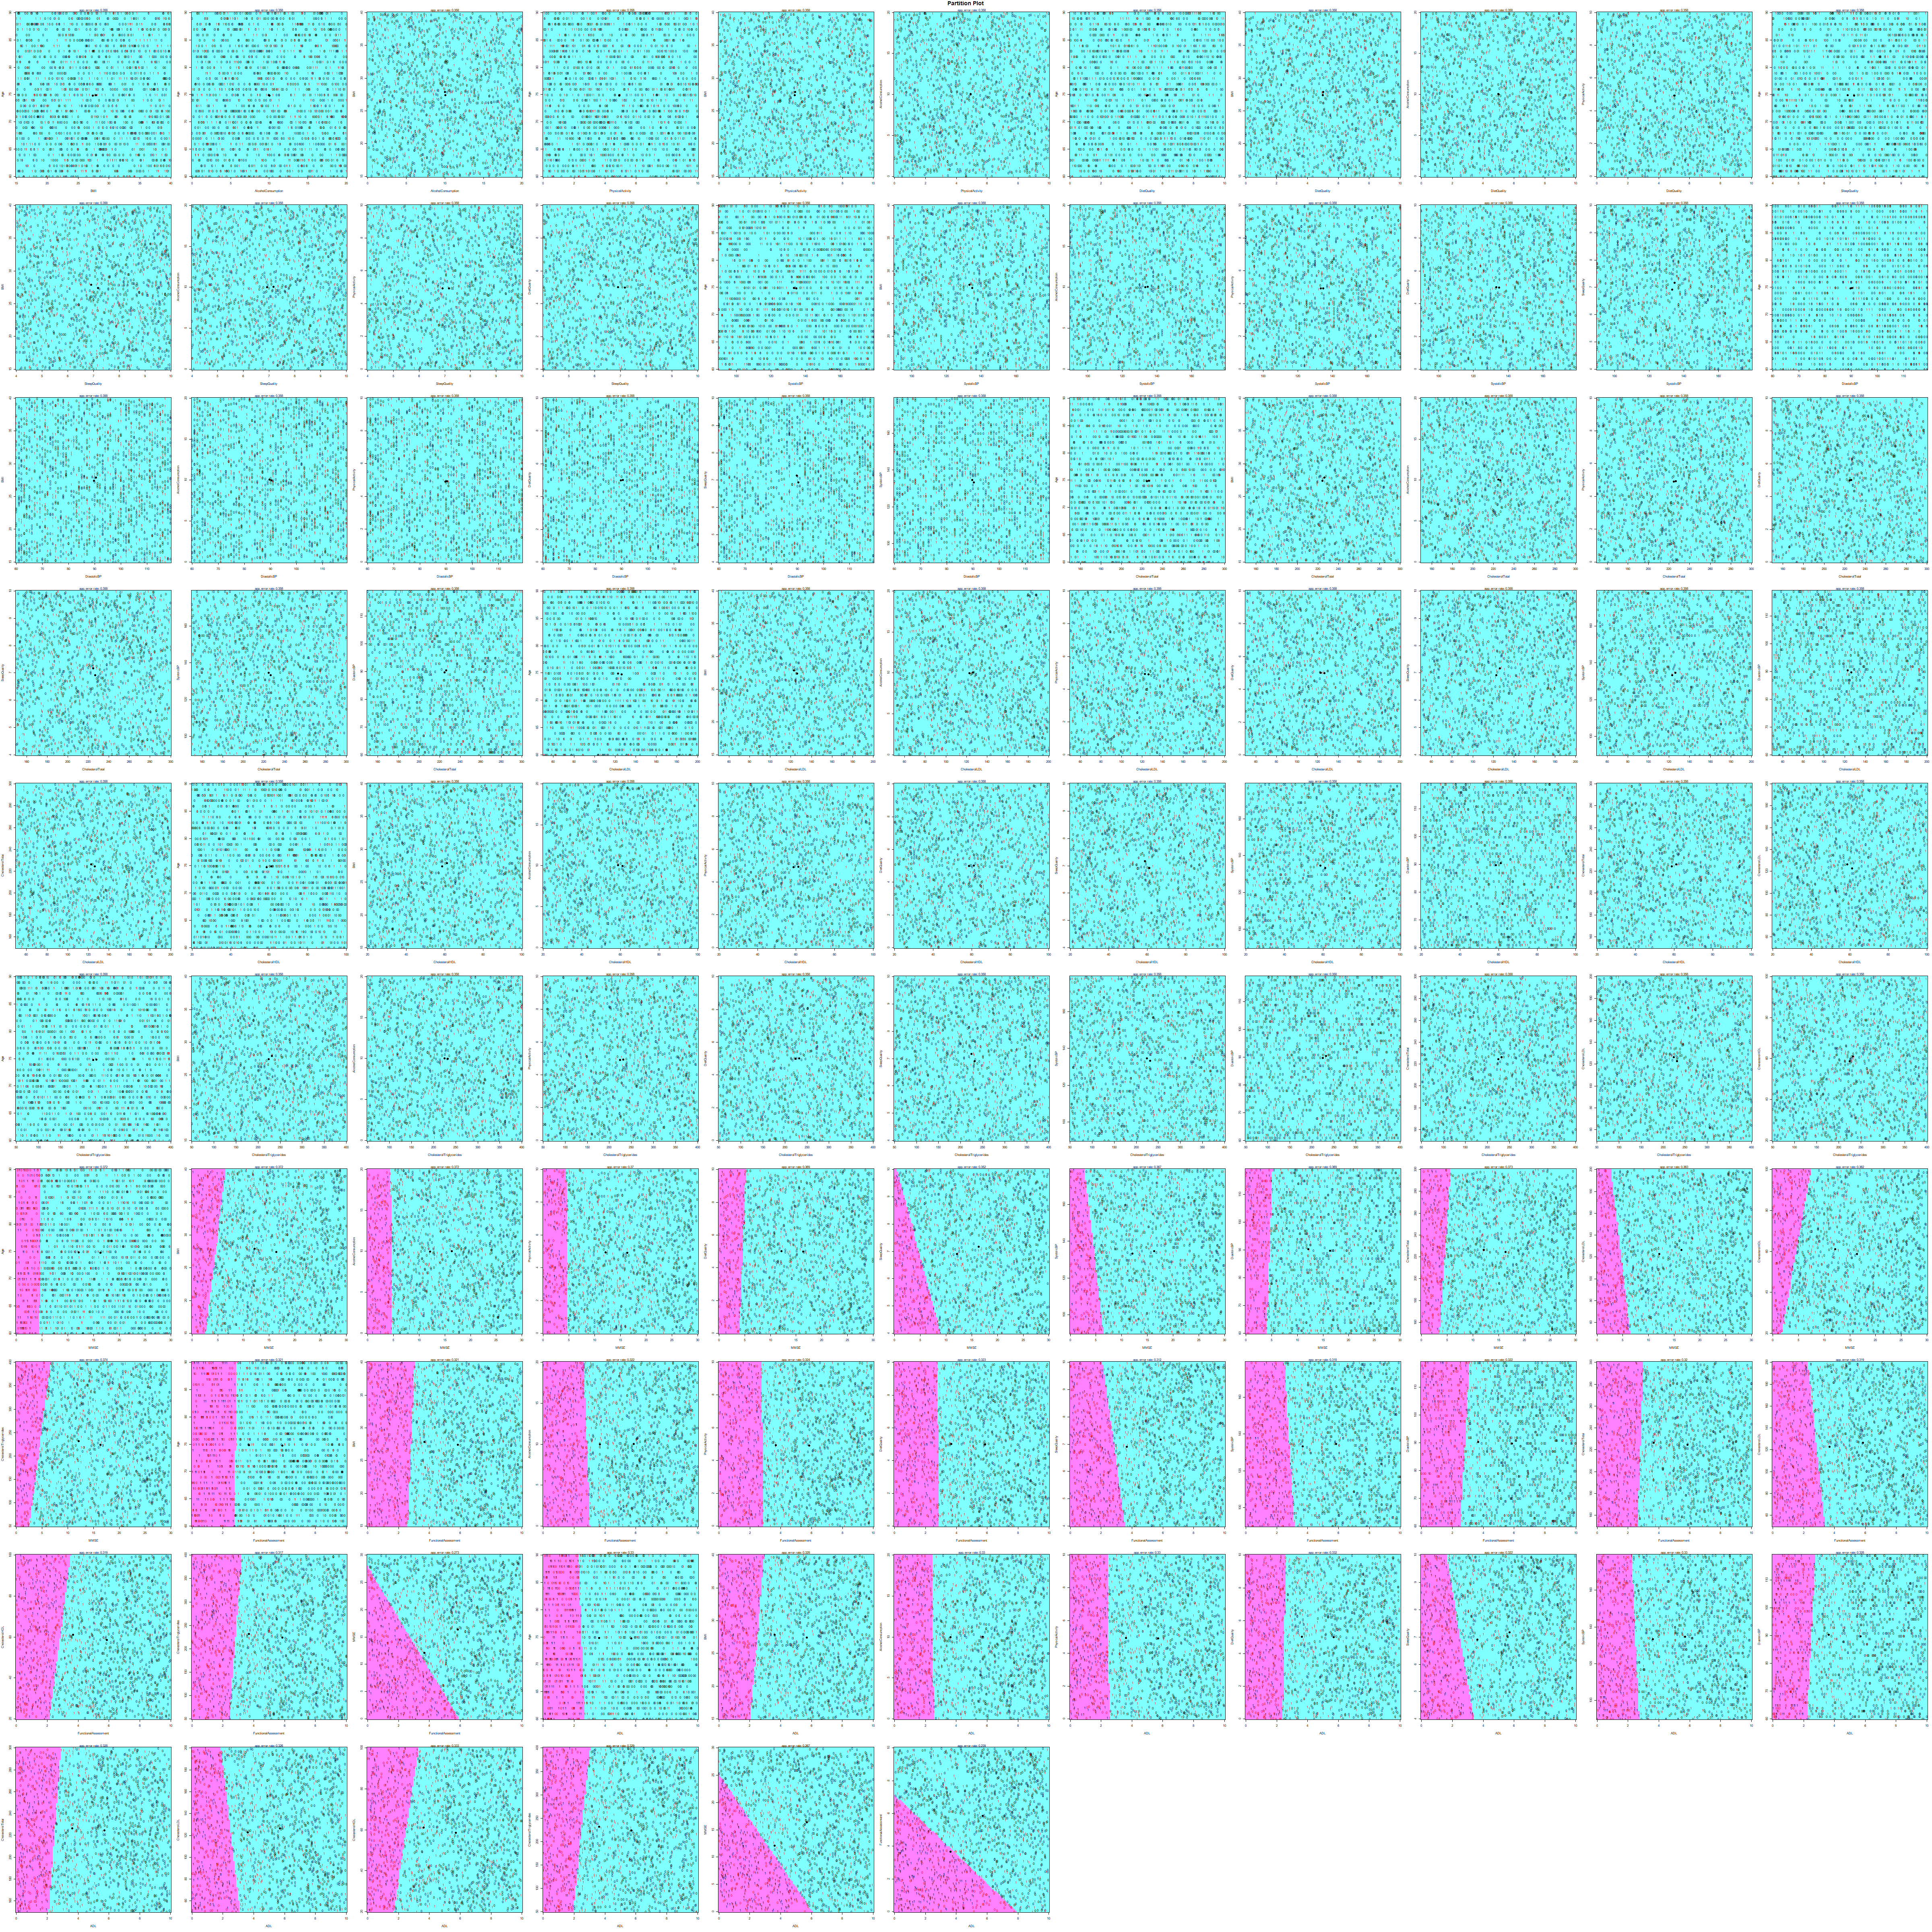
\includegraphics[width = 0.8\textwidth]{PartitionLDA.png}
\end{center}

The figure displays that among the 105 possible partition plots for LDA, only 39 paris show clear separation between AD and Non-AD patients. Notably, all of these 39 plots include at least one the following
variables: MMSE, Functional Assessment, or ADL. This suggest that these three variables may hold the strongest discriminative power  in distinguishing the two groups, as they consistently contribute to visible
class separation. In contrast, the remaining variables, when analyzed in pairs without MMSE, Functional Assessment, and ADL, do not provide distinct visual partitions, implying that these lack stronger linear 
discriminative ability on their own. 

\noindent
\textbf{Figure 8}\\
\textit{Complete Quadratic Class Discrmination of AD and Non-AD Patients}
\begin{center}
    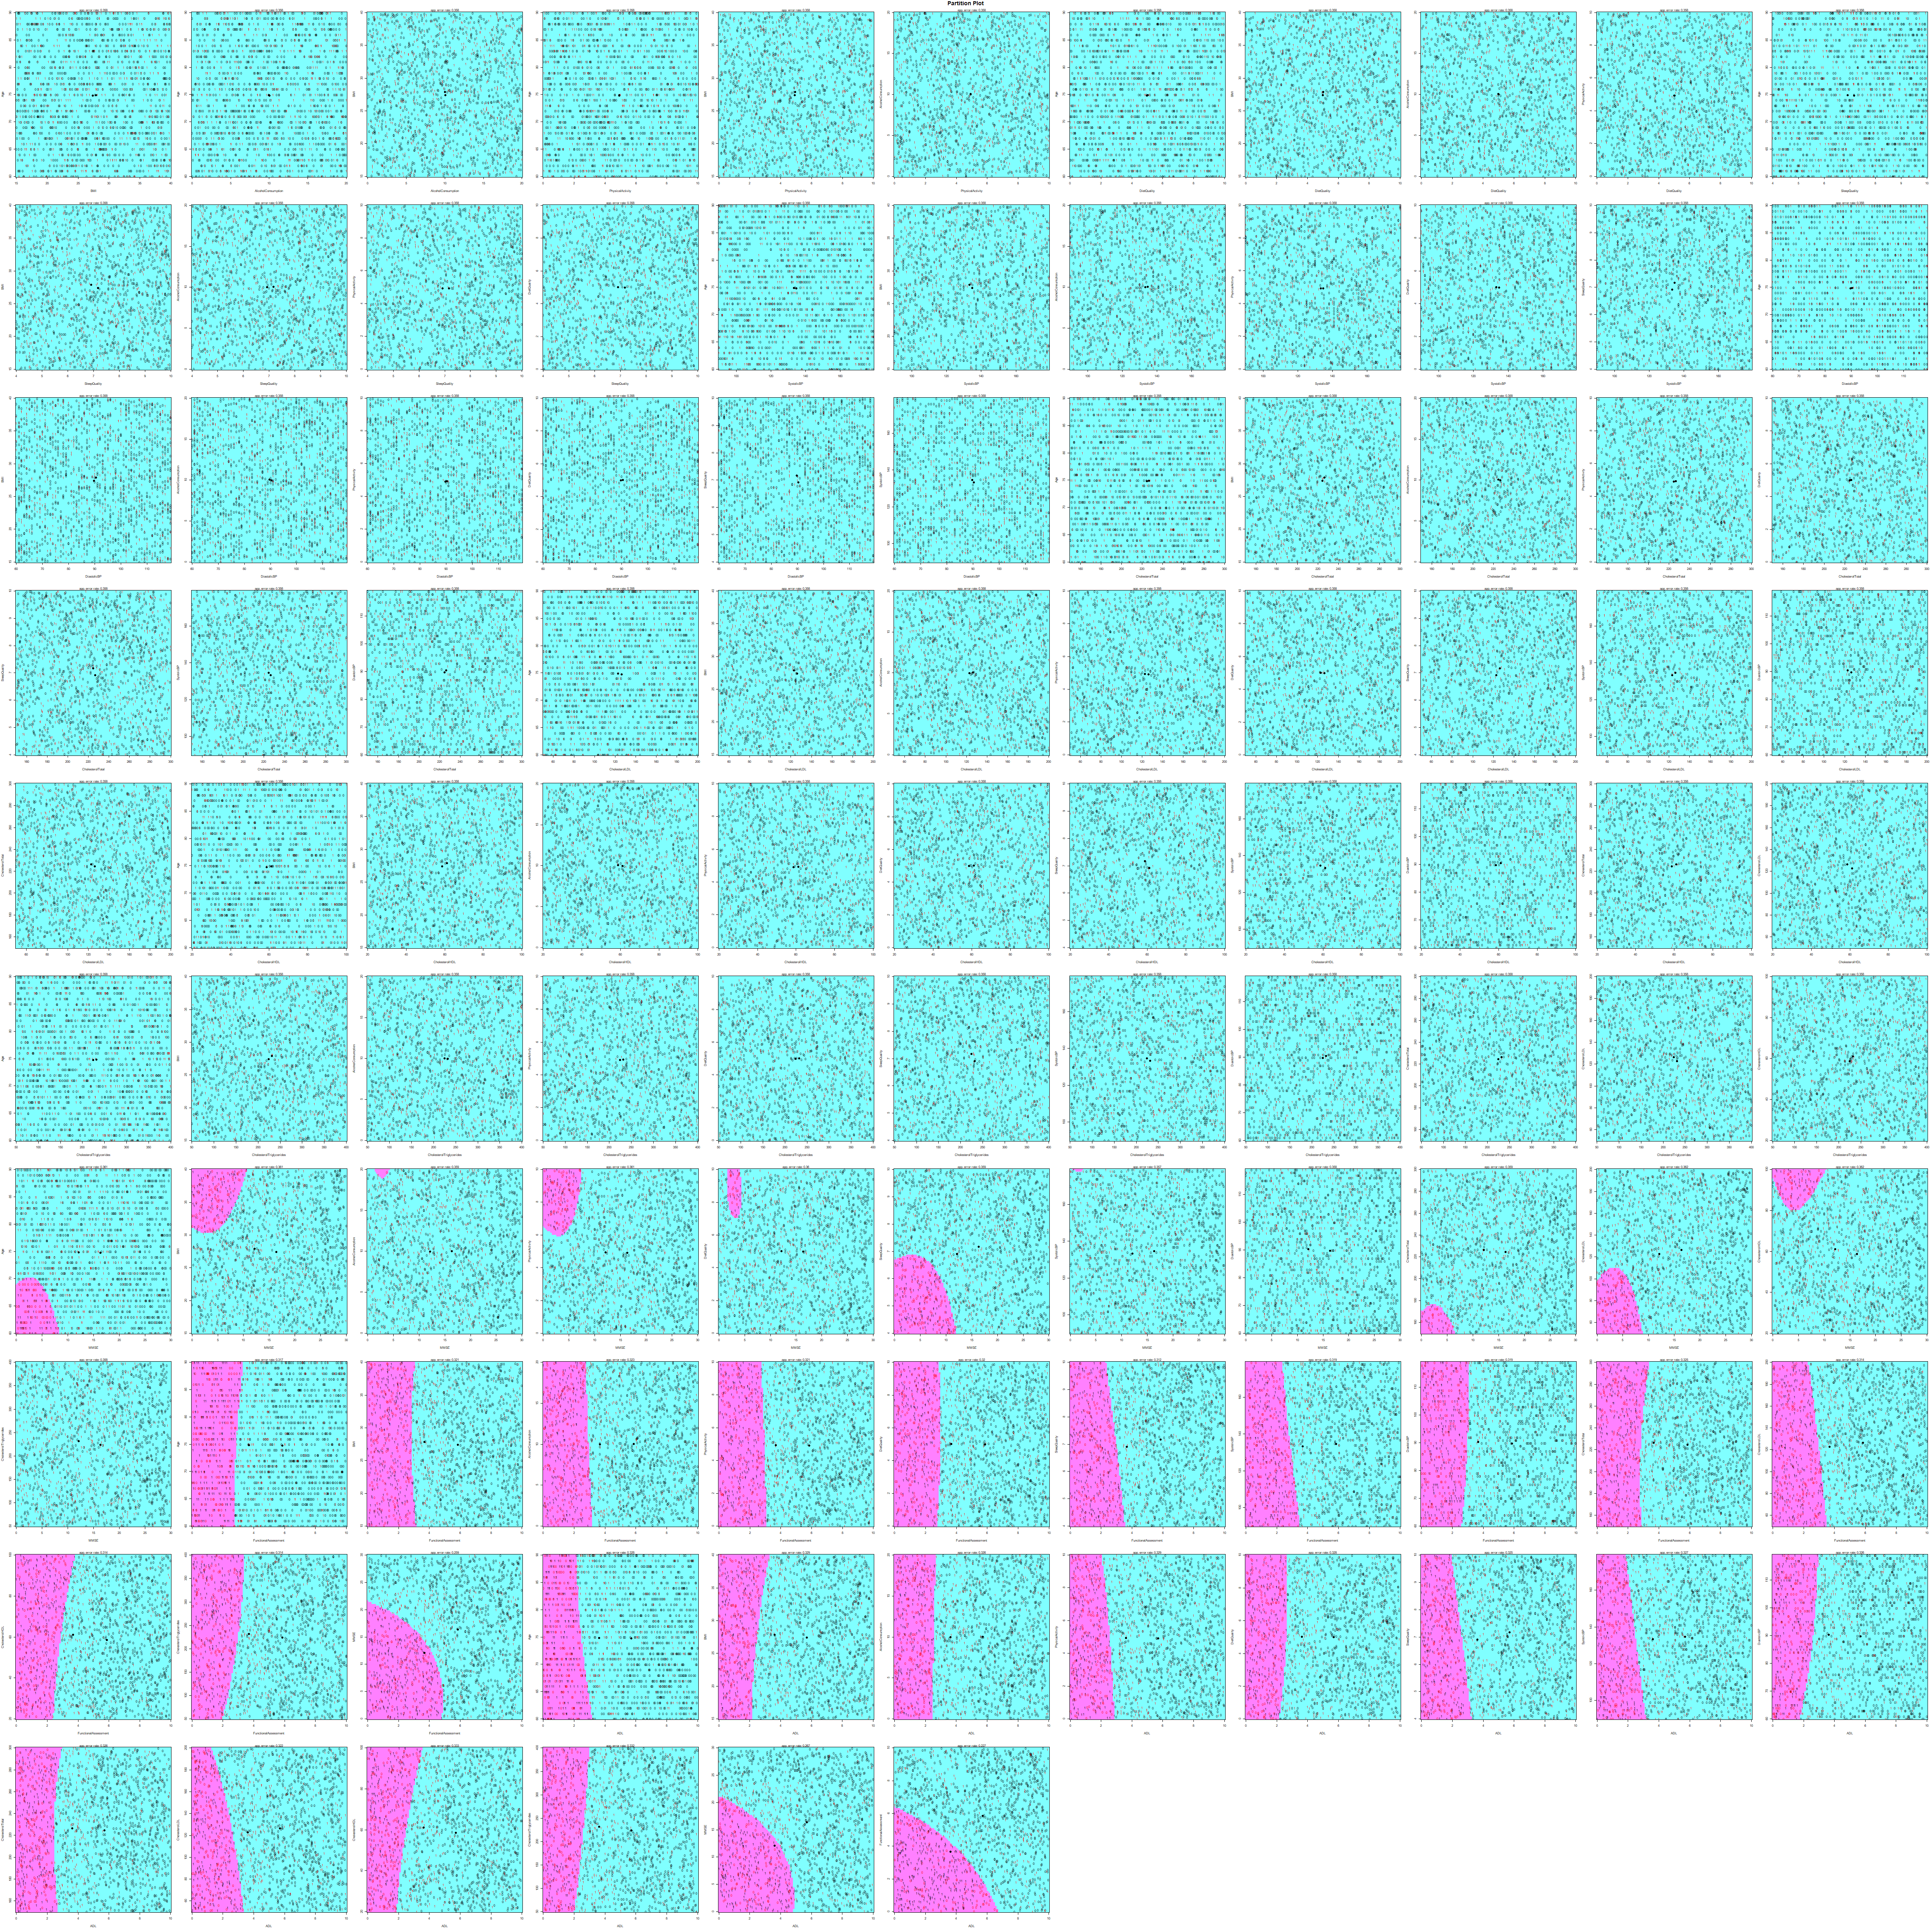
\includegraphics[width = 0.8\textwidth]{PartitionQDA.png}
\end{center}

On the other hand, the figure above shows the 105 possible partition plots for QDA, and almost similar to LDA, only 38 pairs were able to provide distinct separation between diagnosed AD and Non-AD. Speciically, the pairing of MMSE and Diastolic Blood 
Pressure did not show any partition in QDA, as compared to LDA. Through visual inspection, the pairs that include MMSE could only partition smaller and limited regions. This could mean that its effect on distinguishing AD and Non-AD patients may not be consistent 
across all values through QDA. Instead, its discriminative ability might be more pronounced in specific subgroups or at extreme values, which in this case are low MMSE scores, rather than across the entire scale range. This simply means that while its relevant in distinguishing, 
MMSE might not be a standalone predictor in nonlinear classification method. 

\subsubsection{RFE-Reduced Linear and Quadratic Discriminant Models}
\textbf{Figure 9}\\
\textit{Root Mean Squared Error Comparison of Increasing Number of Features}
\begin{center}
    \includegraphics[width = 0.8\textwidth]{Required Number of Features.png}
\end{center}

To determine the optimal number of features for discriminating between AD and Non-AD patients, as shown in figure 9, the error metrics of each model is evaluated as the number of features increases. A significant decline in error is observed after testing the model with three features. Beyond this, the model's error
stabilized, with values consistently close to 0.35. Thus, the reduced model for both LDA and QDA should only have at least three features as predictors to achieve lower error measures and stability. 

\noindent
\textbf{Figure 10} \\
\textit{Recursive Feature Comparison by Importance}
\begin{center}
    \includegraphics[width = 0.8\textwidth]{RFE Feature Selection.png}
\end{center}

Using the same caret algorithm, variable importance is determined using RFE. In figure 10, MMSE, Functional Assessments, and ADL play a significant role in differentiating AD and Non-AD patients, which is consistent with the findings from the density distributions of cognitive and functional assessment and from the complete model of the previous 
discussions. Aside from these three, other variables have no substantial contribution to the distinction of AD and Non-AD patients as evident on the graph. 

\noindent
\textbf{Figure 11} \\
\textit{RFE-Reduced Linear Class Discrimination Model of AD and Non-AD Patients}
\begin{center}
    \includegraphics[width = 0.8\textwidth]{LDA_RFE.png}
\end{center}

Consequently, using the reduced number of features and the variables with the highest importance in figures 9 and 10, respectively, figure 11 displays the linear discrimination of AD patients and Non-AD patients. Compared to the full mdel, all partition pairs in the RFE-reduced linear model 
captured the distinct separation between the two classes. However, the combination of pairings was reduced to three. 

\noindent
\textbf{Figure 12} \\ 
\textit{RFE-Reduced Quadratic Class Discrimination Model of AD and Non-AD Patients}
\begin{center}
    \includegraphics[width = 0.8\textwidth]{QDA_RFE.png}
\end{center}

Similar trends can be observed in the quadratic discrimination of AD patients and Non-AD patients. All partition pairs in the reduced quadratic model captured the nonlinear distinct separation between the two classes. However, consistently, the combination of pairings was reduced to three. 

\subsubsection{Lasso Regression-Reduced Linear and Quadratic Discriminant Models}
\textbf{Figure 13} \\ 
\textit{Lambda Regularization by Feature Coefficients}
\begin{center}
    \includegraphics[width = 0.8\textwidth]{Coefficient vs Log Lambda.png}
\end{center}

The logarithm of lambda controls the regularization strength of the coefficients for feature reduction. As the value of lambda increases, more coefficients shrink towards zero which indicates that more features are being penalized by the model. Based on the graph, along lambda values of -5 to -3, the model 
achieves the best trade-off between coefficient shrinkage and performance. 

\noindent
\textbf{Figure 14}\\
\textit{Binomial Deviance and Logarithmic Lambda}
\begin{center}
    \includegraphics[width = 0.8\textwidth]{Binomial Deviance vs Log Lambda.png}
\end{center}

Upon cross-validated, figure 9 displays the error rate of the lambda values as it increases. Ther red dot are the mean coefficients and vertical lines are its error rates. As the lambda value increases the error rate is also increasing, shrinking the coefficients down to zero. 

\noindent
\textbf{Figure 15}\\
\textit{Feature Importance based on the Optimal Lambda}
\begin{center}
    \includegraphics[width = 0.8\textwidth]{Lasso Feature Selection.png}
\end{center}

Thus, based on the optimal lambda from the lasso regression, ADL, Functional Assessments, MMSE, and Sleep Quality were the top four coefficients compared among the features who almost shrunk to zero. It implies that these four variables contribute the most in discriminating AD patients and Non-AD patients. 

\noindent
\textbf{Figure 16} \\
\textit{Lasso-Reduced Linear Class Discrimination of AD and Non-AD Patients}
\begin{center}
    \includegraphics[width = 0.8\textwidth]{Lasso_Reduced_LDA.png}
\end{center}

Tama na please. 

\noindent
\textbf{Figure 17} \\
\textit{Lasso-Reduced Quadratic Class Discrimination of AD and Non-AD Patients}
\begin{center}
    \includegraphics[width = 0.8\textwidth]{Partimat_QDA_Lasso.png}
\end{center}

Babasahin mo ba to pj

\subsection{Classification Metrics Comparisons of LDA and QDA Models}
\textbf{Figure 18} \\
\textit{Model Accuracies Across 10-Folds}
\begin{center}
    \includegraphics[width = 0.8\textwidth]{Accuracy_Line_plots.png}
\end{center}

Amazing




\newpage
\section{CHAPTER V \\ CONCLUSION AND RECOMMENDATION}

\subsection{Summary of Findings}
\subsection{Recommendations}

\newpage
\raggedleft
\defbibheading{bibliography}[\refname]{\section*{\raggedleft#1}}
\printbibliography

\end{document}